\documentclass[a4paper,12pt]{article}
\usepackage[a4paper,margin=0.7in]{geometry}
\usepackage[spanish]{babel}
\usepackage[utf8]{inputenc}
\usepackage[T1]{fontenc}
\usepackage{amsmath}
\usepackage{cite}
\usepackage{graphicx}
\usepackage{float}

\title{Medición de Distancias Utilizando la Ley del Inverso Cuadrado}
\author{Manuel A. García \\ \texttt{mangarciama@unal.edu.co}}

\begin{document}

\maketitle

\begin{abstract}
Este estudio evalúa la precisión en la medición de distancias mediante el uso de la ley del inverso cuadrado de la luz, utilizando farolas como analogía de velas estándar. Las imágenes capturadas con una cámara digital se analizaron para medir flujos luminosos, y se calcularon distancias antes y después de la corrección propuesta. Los resultados muestran que la aplicación de correcciones de luminosidad reduce significativamente los errores. 
\end{abstract}

\section{Introducción}

Medir la distancia permite relacionar datos observacionales con propiedades intrínsecas, como el tamaño físico o la luminosidad intrínseca de un objeto celeste \cite{poessel2016}. Para objetos más allá del sistema solar, los astrónomos dependen de las velas estándar, cuerpos cuya luminosidad se conoce o puede inferirse a partir de otras propiedades observables.

\subsection{Velas estándar y la ley del inverso cuadrado}

La ley del inverso cuadrado establece que el flujo \(F\), o brillo aparente, de un objeto luminoso disminuye con el cuadrado de la distancia \(d\) según:
\begin{equation}
F = \frac{L}{4\pi d^2},
\label{eq:flujo}
\end{equation}
donde \(L\) es la luminosidad intrínseca del objeto \cite{poessel2016}. Este principio permite calcular distancias si se conoce \(L\) y se mide \(F\).

Las velas estándar son objetos cuya luminosidad intrínseca es conocida, lo que las hace herramientas útiles para determinar distancias en astronomía. En este experimento, se emplean luces de calle como una analogía de velas estándar, utilizando una cámara digital para medir su brillo aparente desde distintas distancias \cite{poessel2016}.

Para obtener el flujo de un objeto sin que el ruido de fondo afecte de manera significativa, una buena aproximación es usar la siguiente expresión para realizar el cálculo del flujo del objeto:
\begin{equation}
F_{\text{obj}} = F_0 - p_{\text{bg}} \cdot A
\label{eq:flujo_objeto}
\end{equation}
De esta forma, podemos calcular la distancia a la lámpara \(i\)-ésima con la siguiente relación:
\begin{equation}
d(i) = d(1) \cdot \sqrt{\frac{F(1)}{F(i)}}
\label{eq:d_prelim}
\end{equation}

\subsection{Corrección de variaciones de luminosidad}

Un problema recurrente es la variación intrínseca en la luminosidad de las velas estándar, lo que puede distorsionar las mediciones. La ecuación corregida:
\begin{equation}
d(i) = d_{\text{ref}} \cdot \sqrt{\frac{r(i) \cdot F(1)}{F(i)}},
\label{eq:d_corr}
\end{equation}
ajusta las distancias considerando las variaciones de luminosidad relativa \(r(i)\) y la extinción causada por elementos intermedios, como polvo o árboles \cite{poessel2016}. Esta corrección es fundamental para obtener mediciones más precisas.
\begin{gather}
r(i) = \frac{L(i)}{L(1)} 
\label{eq:r}
\end{gather}

\section{Montaje Experimental}

Para esta actividad, se capturaron imágenes de 8 farolas situadas a lo largo de una calle recta. Se utilizó una cámara Nikon D5600 con un tiempo de exposición de 1/1000 s y una sensibilidad ISO 100. La cámara se colocó a una distancia de 23.6 metros de la primera lámpara. Las imágenes se tomaron en formato RAW para evitar la pérdida de información debido a la compresión de otros formatos como JPG o PNG.

Posteriormente, las imágenes se convirtieron al formato FITS utilizando el programa \texttt{rawtran}, que es ideal para el análisis fotométrico, ya que conserva toda la información necesaria para la medición precisa de los valores de brillo. Las mediciones se llevaron a cabo utilizando el software \texttt{SAOImageDS9}, que permite realizar fotometría para medir el brillo promedio dentro de una región específica de la imagen, así como el valor medio del fondo en una región del mismo tamaño.

En cada imagen, se registraron los siguientes valores:
\begin{itemize}
    \item El valor promedio del flujo de la lámpara.
    \item El valor promedio del flujo del fondo.
    \item El área de la región seleccionada, expresada en píxeles cuadrados.
\end{itemize}

Estos valores se utilizaron para calcular el brillo corregido de cada farola, siguiendo el método descrito en la sección anterior.

\begin{figure}[H]
    \centering
    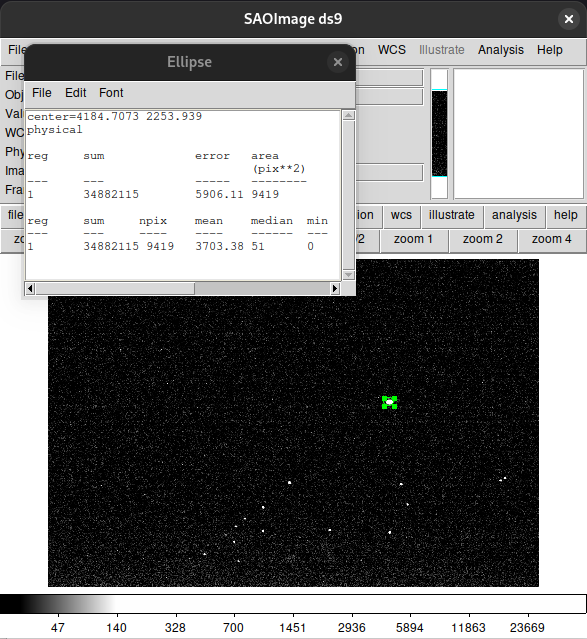
\includegraphics[width=0.45\textwidth]{ds9.png}
    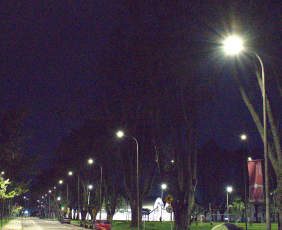
\includegraphics[width=0.5\textwidth]{lamp_reference.png}
    \caption{Captura de pantalla del software \texttt{SAOImageDS9} mostrando la medición de una de las lámparas y la imagen de referencia de las lámparas.}
    \label{fig:saods9}
\end{figure}



\section{Resultados y Analisis}
Con las mediciones realizadas se obtuvieron los siguientes datos:
\begin{table}[H]
\centering
\begin{tabular}{|c|c|c|c|c|}
\hline
\textbf{\# Lampara} & \textbf{F\_mean} & \textbf{F\_bg\_mean} & \textbf{Area} $[px^2]$ & \textbf{d\_real} $[m]$ \\ \hline
1 & 6474.11 & 11.24 & 5378 & 23.6 \\ \hline
2 & 432.81  & 9.22  & 1618 & 47.6 \\ \hline
3 & 192.97  & 10.30 & 1235 & NaN  \\ \hline
4 & 136.15  & 11.13 & 756  & NaN  \\ \hline
5 & 108.89  & 10.81 & 832  & NaN  \\ \hline
6 & 44.75   & 11.26 & 538  & NaN  \\ \hline
7 & 21.87   & 11.15 & 541  & NaN  \\ \hline
8 & 22.10   & 10.14 & 486  & NaN  \\ \hline
\end{tabular}
\caption{Tabla de datos las mediciones.}
\label{tab:lamps}
\end{table}
Usando la ecuacion \ref{eq:flujo} en la ecuacion \ref{eq:r} podemos escribir el termino de correccion en funcion del flujo y la distancia. 
\begin{equation}
  r(i) = \frac{d(i)^2 F(i)}{d(1)^2 F(1)}
  \label{eq:r_flujo}
\end{equation}
En el articulo referenciado \cite{poessel2016} se toma una imagen a cada lampara con una distancia fija para obtener las luminosidades necesarias en para la correccion $ r $. En este caso por falta de tiempo se tomo la distancia a la primera y la segunda lampara y se trazó una recta con estos dos puntos para obtener la distancia real a cada lampara y poder reemplazar estos valores en la ec. \ref{eq:r_flujo}. 

Se uso la eq. \ref{eq:flujo_objeto} para obtener el flujo del objeto y la ec. \ref{eq:d_prelim} para hallar una distancia preliminar; tambien se utilizó la ec. \ref{eq:d_corr} para obtener la distancia con correccion obteniendo la siguiente tabla:
\begin{table}[H]
\centering
\begin{tabular}{|c|c|c|c|c|c|c|c|}
\hline
\textbf{Lamp} & \textbf{d\_real} & \textbf{F\_obj} & \textbf{d\_prelim} & \textbf{error\%} & \textbf{r} & \textbf{d\_adjusted} & \textbf{error\%} \\ \hline
1 & 23.60 & 6462.87 & 23.06 & 2  & 1.00 & 23.06 & 2  \\ \hline
2 & 44.10 & 423.59  & 90.07 & 104 & 0.21 & 41.24 & 6  \\ \hline
3 & 64.60 & 182.67  & 137.16 & 112 & 0.19 & 60.18 & 6  \\ \hline
4 & 85.10 & 125.02  & 165.80 & 94  & 0.23 & 79.63 & 6  \\ \hline
5 & 105.60 & 98.09  & 187.18 & 77  & 0.28 & 99.11 & 6  \\ \hline
6 & 126.10 & 33.49  & 320.33 & 154 & 0.16 & 129.25 & 2  \\ \hline
7 & 146.60 & 10.72  & 566.22 & 286 & 0.11 & 185.07 & 26 \\ \hline
8 & 167.10 & 11.96  & 535.98 & 220 & 0.14 & 200.27 & 19 \\ \hline
\end{tabular}
\caption{Datos de las lámparas con distancias reales, preliminares y ajustadas.}
\label{tab:analisis}
\end{table}

Con esta tabla se realizó la siguiente grafica:
\begin{figure}[H]
    \centering
    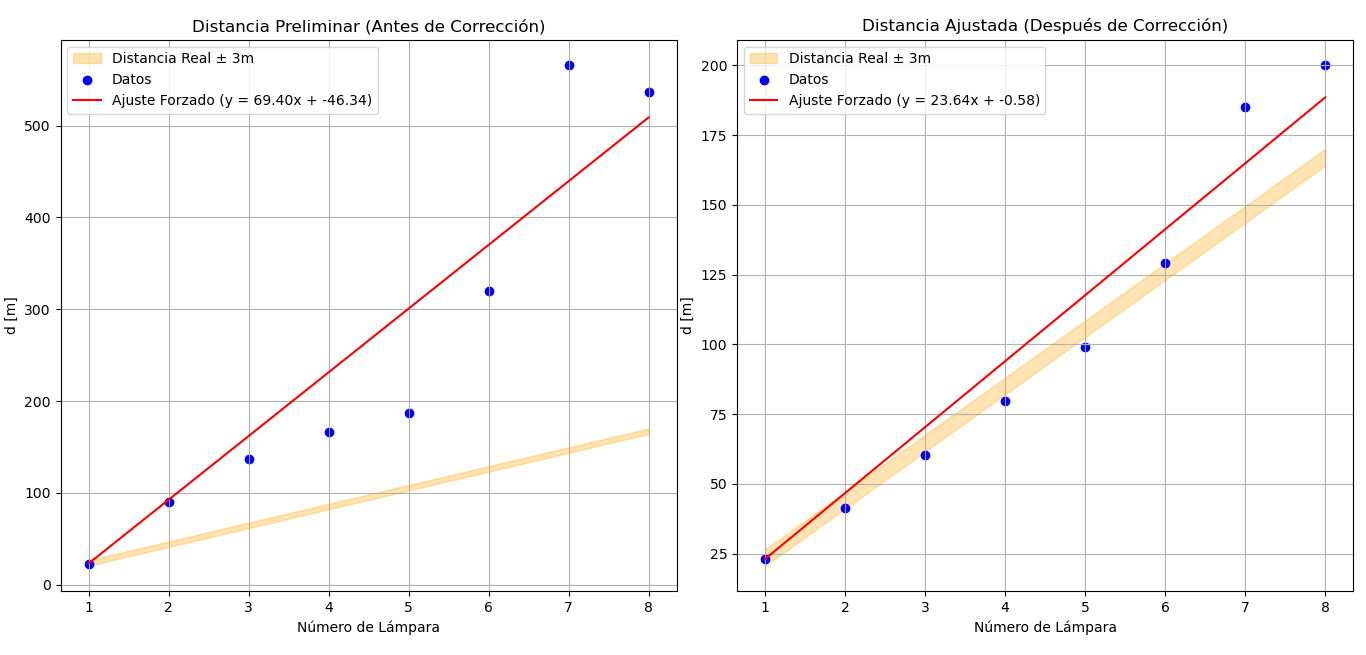
\includegraphics[width=0.85\textwidth]{grafica_analisis.png}
    \caption{Graficas obtenidas con el analisis realizado de la tabla \ref{tab:analisis}}
    \label{fig:analisis2}
\end{figure}
En la figura \ref{fig:saods9} se realizó un ajuste lineal forzado a pasar por el primer punto de los datos para poder apreciar la tendencia de los datos tomados. Se observó que antes de la correccion los datos tomados tienen errores muy grandes de hasta el $ 112\% $ en los primeros datos y de hasta $ 286\% $ en los outlayers. Sin embargo luego de la correccion se obtienen valores muy cercanos a los esperados siendo el error mas grande de $ 26\% $ para unos de los outlayers.




\section{Verificacion Ley del Inverso Cuadrado }
Para verificar la ley del inverso cuadrado se realizó el mismo procedimiento que con las lamparas de calle pero con un led en lugar de lamparas. Se tomó una imagen del led cada 10cm para luego realizar el mismo analisis de la seccion anterior. Se obtuvo la siguiente tabla:
\begin{table}[H]
\centering
\begin{tabular}{|c|c|c|c|c|c|c|}
\hline
Lamp & F\_mean & F\_bg\_mean & Area $[px]$ & d\_real $ [cm] $ & d\_prelim $ [cm] $ & error\% \\ \hline
1    & 14171.60 & 49.42   & 29433 & 20.00  & 20.00 & 0.00  \\ \hline
2    & 18692.70 & 84.19   & 13258 & 30.00  & 25.96 & 13.47 \\ \hline
3    & 11127.90 & 44.03   & 12922 & 40.00  & 34.07 & 14.82 \\ \hline
4    & 6716.28  & 42.48   & 12816 & 50.00  & 44.09 & 11.82 \\ \hline
5    & 6404.19  & 40.53   & 9265  & 60.00  & 53.10 & 11.49 \\ \hline
6    & 5130.12  & 36.68   & 8446  & 70.00  & 62.17 & 11.19 \\ \hline
7    & 4493.05  & 37.63   & 7494  & 80.00  & 70.57 & 11.79 \\ \hline
8    & 3143.30  & 39.34   & 8419  & 90.00  & 79.76 & 11.37 \\ \hline
\end{tabular}
\caption{Datos de las lámparas con distancias reales y las calculadas por la ley del inverso cuadrado.}
\label{tab:analisis2}
\end{table}
Con estos datos se contruyó la siguiente grafica:
\begin{figure}[H]
    \centering
    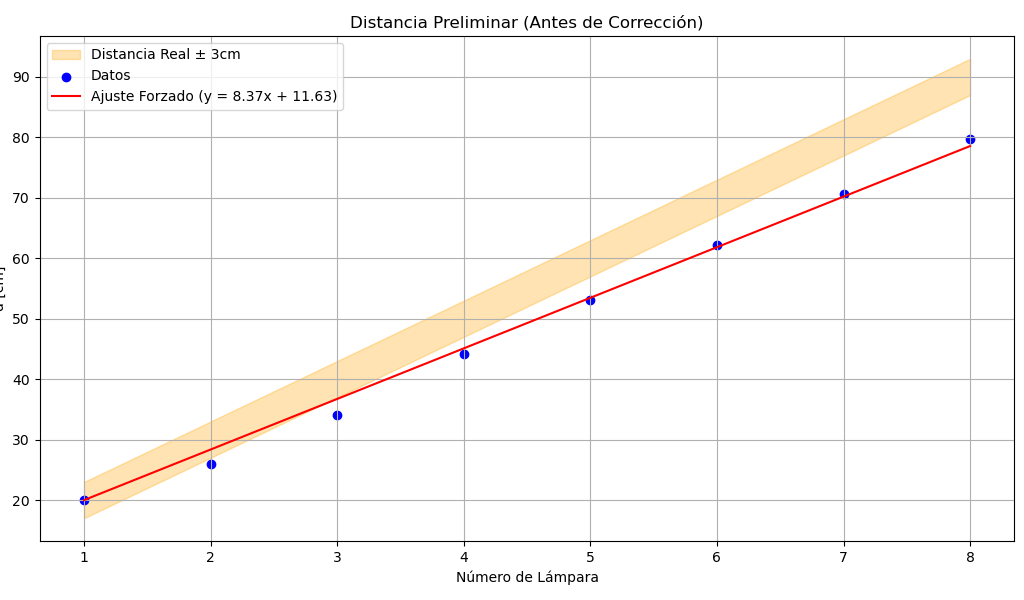
\includegraphics[width=0.85\textwidth]{grafica_analisis2.png}
    \caption{Graficas obtenidas con el analisis realizado de la tabla \ref{tab:analisis2}}
    \label{fig:analisis2}
\end{figure}




\section{Conclusiones}
El uso de la ley del inverso cuadrado y las correcciones de luminosidad relativa permiten medir distancias con mayor precisión, incluso en condiciones no ideales. Este método se mostró eficaz para reducir errores de hasta un \(286\%\) a valores más manejables, mejorando la confiabilidad de las mediciones.




\bibliographystyle{plain}
\bibliography{references}

\end{document}
